\Askhsh{16099_SOLUTION}{1}
\begin{ylh}{1}
    \item [Στην εικόνα παρουσιάζεται η λύση μιας άσκησης γεωμετρίας.]
\end{ylh}
\begin{wrapfigure}[15]{r}{6.5cm} % Adjust number of lines and width as needed
    \centering
    \begin{tikzpicture}[scale=0.18] % Adjust scale to fit the diagram
        % Define points B, A, D
        \tkzDefPoint(0,0){B}
        \tkzDefPoint(-24,0){A} % AB = 24 (calculated later in the solution)
        \tkzDefPoint(16,0){D}
        
        % Define points G (Gamma) and E on the y-axis
        % Based on calculations: BΓ = 12√5 ≈ 26.83, BE = 8√5 ≈ 17.89
        \tkzDefPoint(0,26.83){G} % Gamma
        \tkzDefPoint(0,17.89){E} % Epsilon
        
        % Draw segments
        \tkzDrawSegments(A,B B,D G,E) % Draw main lines: A-B-D and G-B-E (vertical line)
        \tkzDrawSegments(A,G E,D) % Draw hypotenuses
        
        % Mark the right angle at B
        \tkzMarkRightAngle[size=1.5mm](A,B,G)
        
        % Label points
        \tkzLabelPoint[left](A){A}
        \tkzLabelPoint[below](B){B}
        \tkzLabelPoint[right](D){$\Delta$}
        \tkzLabelPoint[above left](G){$\Gamma$}
        \tkzLabelPoint[right](E){E} % Position E label slightly to the right for clarity
        
        % Label segment lengths
        \tkzLabelSegment[above left](A,G){36}
        \tkzLabelSegment[above right](E,D){24}
        \tkzLabelSegment[below](B,D){16}
    \end{tikzpicture}
\end{wrapfigure}
\begin{alist}
\item Τα τρίγωνα $\text{AB}\Gamma$ και $\Delta\text{BE}$ έχουν $\hat{\text{A}} = \hat{\Delta}$ (από υπόθεση) και $\text{A}\hat{\text{B}}\Gamma = \Delta\hat{\text{B}}\text{E} = 90^\circ$. Αφού τα τρίγωνα έχουν δύο γωνίες τους ίσες μία προς μία, τότε θα είναι όμοια.
\item Τα τρίγωνα $\text{AB}\Gamma$ και $\Delta\text{BE}$ είναι όμοια, οπότε θα έχουν τις ομόλογες πλευρές τους ανάλογες. Οι ομόλογες πλευρές των δύο τριγώνων σημειώνονται στον ακόλουθο πίνακα:

\[
\begin{tabular}{|l|c|c|c|}
\hline
\multicolumn{1}{|l|}{} & \multicolumn{3}{c|}{Ίσες γωνίες} \\
\cline{2-4}
\multicolumn{1}{|l|}{} & $\hat{\text{A}} = \hat{\Delta}$ & $\text{A}\hat{\text{B}}\Gamma = \Delta\hat{\text{B}}\text{E} = 90^\circ$ & $\text{A}\hat{\Gamma}\text{B} = \Delta\hat{\text{E}}\text{B}$ \\
\hline
Απέναντι πλευρά στο τρίγωνο $\text{AB}\Gamma$ & $\text{B}\Gamma$ & $\text{A}\Gamma$ & $\text{AB}$ \\
\hline
Απέναντι πλευρά στο τρίγωνο $\Delta\text{B}\text{E}$ & $\text{BE}$ & $\text{E}\Delta$ & $\text{B}\Delta$ \\
\hline
\end{tabular}
\]
Έτσι έχουμε:
\[ \frac{\text{A}\Gamma}{\text{E}\Delta} = \frac{\text{AB}}{\text{B}\Delta} \text{ ή } \frac{36}{24} = \frac{\text{AB}}{16} \text{ ή } \text{AB} = \frac{36 \cdot 16}{24} = 24 \]
\end{alist}